\subsection*{Game Story}

\subsubsection*{Synopsis}

\paragraph{Introduction}
Years after the Battle of Hogwarts, Delphini Lestrange meets her stepfather, who convinces her to embark in a mission into the past in order to save her family. She goes back thanks to a gifted timeturner and meets Minerva.

\paragraph{Daily life at Hogwarts}
School starts and Minerva first meets Delphini as a new student in the Black Lake whereabouts. During the first part of the year Minerva deepens her relationship with Delphini as they meet toghether with Myrtle to study.

\paragraph{Petrified}
Suddenly some students are found petrified around the school. The air is full of tension, and everything escalates when Myrtle is found petrified too. Minerva and Delphini start to investigate.

\paragraph{To Trust or Not to Trust}
Tom Riddle accuses Hagrid of keeping in secret the monster who caused all the deaths. When Aragog was discovered, Hagrid is banished from the school despite Albus Dumbledore defending him. Delphini becomes suspicious of both Tom and Dumbledore. Hoever, she only talks to Minerva about the latter.

\paragraph{Final Confrontation}
Minerva and Delphini reach Dumbledore's office, either to confront him (Minerva trusts Delphini), tell him the truth (Minerva trusts Dumbledore, Delphini's friendship is strong), or fight each other (Delphini's friendship is weak).

\subsubsection*{Story}

\paragraph{Background}
Few years after the Battle of Hogwarts Delphini Lestrange is visited by her step-father Rodolphus Lestrange, who escaped from Azkaban to meet her and reveal that she was Voldemort's daughter.
Fast forward to 2007, Delphini learned a lot from her stepfather. He convinced her that had Voldemort won the First Wizarding War, the Second one would not have happened, and her family would still be alive. During her birthday, Rodolphus gifted her a Timeturner, a falsified Hogwarts Acceptance Letter for the year 1942, a mission, to find some powerful student to help Tom Riddle in the First Wizarding War, and a hope: to prevent the death of her family. 

\paragraph{Introduction}
It's Minerva's 7th year at Hogwarts. She became acquainted with a new student: Delphini. Minerva had few friends; one was Myrtle Warren.

\paragraph{Rising Action}
Minerva quickly got closer to Delphini, they started studying together. Sometimes Delphini would surprise her teaching her things she did not know. Delphini also helped her getting more familiar with the Animagus powers to which she had been introduced by her Transfiguration teacher, Dumbledore.
Meanwhile Delphini met her father, Tom Riddle. She told him about his future defeat during the First Wizarding War, then offered to help him winning it.
Dumbledore was secretly keeping an eye on Delphini, having found out her letter was falsified, and having troubles discovering anything about her past.

\paragraph{Climax}
One day Delphini told Riddle about Slytherin's Chamber of Secrets. Riddle opened the Chamber and found the Basilisk. In the following days students were found petrified, causing an atmosphere of fear. All escalated when Myrtle was found petrified.

\paragraph{Falling Action}
Minerva and Delphini started to investigate about what we're going on. Delphini began suspecting her father was behind the attacks, but never revealed these suspects.
When Tom Riddle found out about Hagrid keeping in secret an Acromantula, Aragog, in order to prevent the school from being shut he reported that to the headmaster of the school, Dippet, implying Aragog was behind the attacks. Hagrid was then expelled,  and the school remained open.
Riddle never told Delphini the truth, and she started suspecting Hagrid was the real villain. She began pushing the investigation towards that path  and started pointing out how Dumbledore kept defending Hagrid.

\paragraph{Resolution}
At that point Minerva had to make a choice: \\

\textbf{side with Delphini}
They go confront Dumbledore, who by then found out the truth about Delphini. Dumbledore tries to attack Delphini but retains from harming Minerva despite Minerva helping her friend. Finally, Minerva disarms Dumbledore, when suddenly Tom Riddle reaches the room and kills Albus.\\

\textbf{side with Dumbledore; her relationship with Delphini is strong}
Delphini will follow Minerva to Dumbledore's office and reveal the truth about her admission, her mission, and reveal her suspicion about Riddle being behind the attacks. The three would be interrupted by Riddle, and a fight would start; as soon as Riddle realizes he is going to lose, he escapes in a cloud of smoke.\\

\textbf{side with Dumbledore; her relationship with Delphini is weak}
Delphini will follow Minerva to Dumbledore's office pretending to be on her side, only to suddenly attack them both together with Riddle as soon as he walked past the door behind them.

\subsubsection*{Story flowchart}

\begin{figure}[H]
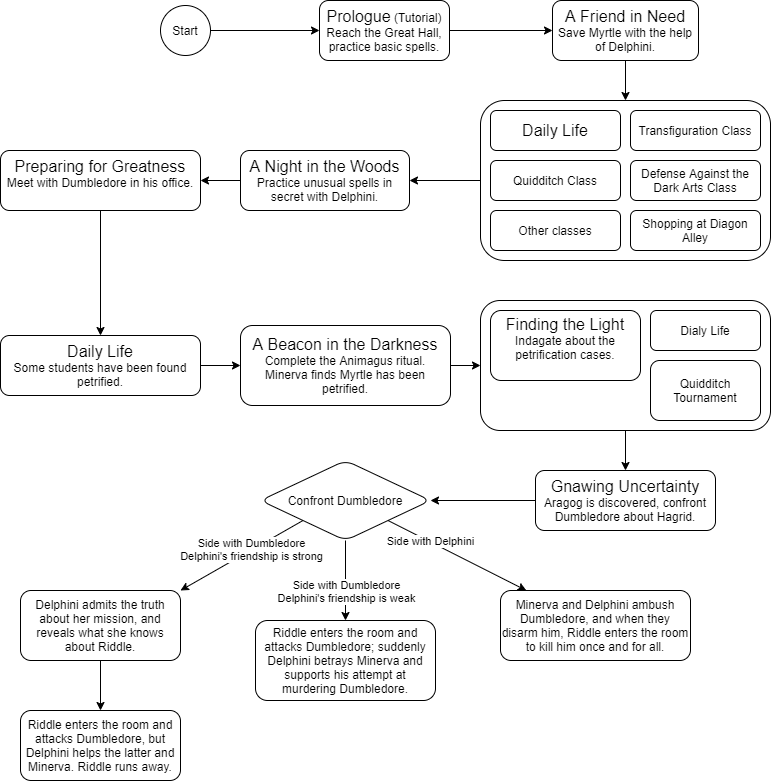
\includegraphics[max width=\textwidth]{../Pictures/Story/Story_flowchart.png}
\end{figure}

\pagebreak